\subsection{FET}
El transistor JFET (transistor de efecto de campo de unión) es un tipo de FET
que opera con una unión \emph{pn} polarizada en inversa para controlar corriente
en un canal. Según su estructura, los JFET caen dentro de cualquiera de dos
categorías, de canal \emph{n} o de canal \emph{p}. Cada extremo del canal tiene
una terminal; el \textbf{drenaje} se encuentra en el extremo superior y la
\textbf{fuente} en el inferior. Se forma un canal donde se conecta la terminal
de la \textbf{compuerta} como se muestra en la \textbf{figura~\ref{figura06}}
junto a sus símbolos esquemáticos \cite{Floyd}.

\begin{figure}[!ht]
\centering
\includegraphics[scale=0.30]{diagramas/figura06.eps}
\caption{Tipos de transistores JFET y sus símbolos estándar.}
\label{figura06}
\end{figure}

Ambos tipos de FET se controlan por una tensión entre la compuerta y la fuente.
La fuente y el drenaje de un FET se pueden intercambiar sin afectar la operación
del transistor.

Cuando se conecta un transistor JFET a un circuito, como se muestra en la
\textbf{figura~\ref{figura07}}, se aplica una fuente de tensión $V_{\text{DD}}$
al drenaje (análoga a la fuente de tensión $V_{\text{CC}}$ para el BJT) y se
envía a tierra. Una fuente de tensión de compuerta $V_{\text{GG}}$ se aplica a
la compuerta (análoga a $V_{\text{BB}}$ para el BJT).

$V_{\text{DD}}$ proporciona una tensión drenaje a fuente $V_{\text{DS}}$ que
provoca una corriente de drenaje $I_{\text{D}}$ del drenaje a la fuente. La
corriente de drenaje $I_{\text{D}}$ que es idéntica a la corriente de fuente,
existe en el canal rodeado por la compuerta de tipo \emph{p}. La tensión
compuerta a fuente $V_{\text{GS}}$ que es igual a $-V_{\text{GG}}$ crea una
región desértica en el canal que reduce el ancho de este y por tanto aumenta la
resistencia entre drenaje y fuente. Como la unión compuerta-fuente esta
polarizada en inverso, el resultado es una corriente de compuerta nula
\cite{Savant}.

\begin{figure}[!ht]
\centering
\includegraphics[scale=0.30]{diagramas/figura07.eps}
\caption{Circuito de polarización de cd del transistor canal \emph{n}.}
\label{figura07}
\end{figure}

Cuando se incrementa $V_{\text{DS}}$ también aumenta la corriente de drenaje
$I_{\text{D}}$, conforme aumenta $V_{\text{DS}}$ se alcanza un punto donde la
corriente de drenaje alcanza su punto de saturación. Si se aumenta
$V_{\text{DS}}$ mas allá de este punto $I_{\text{D}}$ permanece constante. El
valor de la corriente de saturación de drenaje con $V_{\text{GS}} = 0$ es un
parámetro importante y se denomina \textbf{corriente de drenaje de saturación}
($I_{\text{DSS}}$).

El FET es un dispositivo controlado por tensión y se controla mediante
$V_{\text{GS}}$. Conforme se incrementa $V_{\text{GS}}$ (más negativo para un
canal \emph{n} y más positivo para un canal \emph{p}) se cierra para un valor
menor que $I_{\text{D}}$. Por tanto, para el JFET de canal \emph{n} la
$I_{\text{D}}$ máxima se reduce desde $I_{\text{DSS}}$ conforme $V_{\text{GS}}$
se hace mas negativo. Si $V_{\text{GS}}$ disminuye aun mas (mas negativo), se
alcanza un valor de $V_{\text{GS}}$ después del cual $I_{\text{D}}$ sera cero
sin importar el valor de $V_{\text{DS}}$. Este valor de $V_{\text{GS}}$ se
denomina $V_{\text{GS(corte)}}$ o \textbf{tensión de estrangulamiento}
($V_{\text{p}}$). El valor de $V_{\text{p}}$ es negativo para un JFET de canal
\emph{n} y positivo para un JFET de canal \emph{p} \cite{Savant}.

\subsubsection{Curva característica}
En la \textbf{figura~\ref{figura08}} se muestran las curvas características de
transferencia y la curva característica $I_{\text{D}}-V_{\text{GS}}$ para un
JFET de canal \emph{n}. Se graficaron con el eje $I_{\text{D}}$ común.

\begin{figure}[!ht]
\centering
\includegraphics[scale=0.43]{diagramas/figura08.eps}
\caption{Familia de curvas $V_{\text{CE}}$ contra $I_{\text{C}}$ para varios
valores de $I_{\text{B}}$.}
\label{figura08}
\end{figure}

Un método útil de determinar la curva característica de transferencia es con
ayuda de la siguiente relación (ecuación de \emph{Shockley}):

\begin{equation*}
    \frac{I_{\text{D}}}{I_{\text{DSS}}} \approx
    \left(1 - \frac{V_{\text{GS}}}{V_{\text{p}}}\right)^2
\end{equation*}

Por tanto, solo se necesita conocer $I_{\text{DSS}}$ y $V_{\text{p}}$, y toda la
característica queda determinada.

\subsubsection{Transistor 2N3819}
Para la construcción del amplificador se utilizará el transistor JFET canal
\emph{n} \textbf{2N3819}; la hoja de datos de este transistor se detalla en
el \textbf{cuadro~\ref{cuadro04}} \cite{2N3819}.

\begin{table}[!ht]
\begin{center}
    \begin{tabular}{|c|l|c|c|c|}
    \hline
    \multicolumn{5}{|c|}{\textbf{Valores nominales absolutos máximos}}
    \tabularnewline \hline
    \textbf{Símbolo} &
    \textbf{Parámetro} &
    \multicolumn{2}{|c|}{\textbf{Valor}} &
    \textbf{Unidades}
    \tabularnewline \hline \hline
    $V_{\text{DG}}$ &
    Voltaje drenaje-compuerta &
    \multicolumn{2}{|c|}{$25$} & $V$
    \tabularnewline \hline
    $V_{\text{GS}}$ &
    Voltaje compuerta-fuente &
    \multicolumn{2}{|c|}{$-25$} &
    $V$
    \tabularnewline \hline
    $I_{\text{D}}$ &
    Corriente de drenaje &
    \multicolumn{2}{|c|}{$50$} &
    $mA$
    \tabularnewline \hline
    $I_{\text{GF}}$ &
    Corriente en compuerta en polarización directa &
    \multicolumn{2}{|c|}{$10$} &
    $mA$
    \tabularnewline \hline
    $P_{\text{D}}$ &
    Disipación total del dispositivo &
    \multicolumn{2}{|c|}{$350$} &
    $mW$
    \tabularnewline \hline \hline
    \multicolumn{5}{|c|}{\textbf{Características eléctricas (apagado)}}
    \tabularnewline \hline
    \textbf{Símbolo} &
    \textbf{Parámetro} &
    \textbf{Mín.} &
    \textbf{Máx.} &
    \textbf{Unidades}
    \tabularnewline \hline \hline
    $V_{\text{BR(GSS)}}$ &
    Voltaje de ruptura entre compuerta y fuente &
    $25$ &
    $-$ &
    $V$
    \tabularnewline \hline
    $I_{\text{GSS}}$ &
    Corriente inversa en la compuerta &
    $-$ &
    $2.0$ &
    $nA$
    \tabularnewline \hline
    $V_{\text{GS(off)}}$ &
    Voltaje de corte entre compuerta y fuente &
    $-$ &
    $8$ &
    $V$
    \tabularnewline \hline
    $V_{\text{GS}}$ &
    Voltaje entre la compuerta y fuente &
    $-0.5$ &
    $-7.5$ &
    $V$
    \tabularnewline \hline \hline
    \multicolumn{5}{|c|}{\textbf{Características eléctricas (encendido)}}
    \tabularnewline \hline
    \textbf{Símbolo} &
    \textbf{Parámetro} &
    \textbf{Mín.} &
    \textbf{Máx.} &
    \textbf{Unidades}
    \tabularnewline \hline \hline
    $I_{\text{DSS}}$ &
    Corriente en drenaje con voltaje cero en compuerta &
    $2$ &
    $20$ &
    $mA$
    \tabularnewline \hline
    \end{tabular}
\end{center}
\caption{Hoja de datos parcial 2N3819.}
\label{cuadro04}
\end{table}

\subsubsection{Medición de transistores}
Como en el caso de los transistores BJT, los transistores JFET pueden variar sus
parámetros individualmente en un intervalo determinado por la hoja de datos.

\begin{figure}[!ht]
\centering
\includegraphics[scale=0.04]{diagramas/figura09.eps}
\caption{Transistores 2N3918.}
\label{figura09}
\end{figure}

Debido al alto costo de los transistores JFET solo se cuentan con tres de ellos
como puede verse en la \textbf{figura~\ref{figura09}}, de los cuales se medirán
su corriente de drenaje de saturación ($I_{\text{DSS}}$) y su tensión de
estrangulamiento ($V_{\text{p}}$), con la ayuda del circuito presentado en la
\textbf{figura~\ref{figura10}} \cite{measuring}.

\begin{figure}[!ht]
\centering
\includegraphics[scale=0.30]{diagramas/figura10.eps}
\caption{Circuito para el calculo de $V_{\text{p}}$ y $I_{\text{DSS}}$.}
\label{figura10}
\end{figure}

Los valores obtenidos en la medición son detallados en el
\textbf{cuadro~\ref{cuadro05}} con los cuales pueden hallarse las curvas
características que pueden verse en la \textbf{figura~\ref{curva01}}.

\begin{table}[!ht]
\begin{center}
    \begin{tabular}{|c||c|c|}
    \hline
    No. & $V_{\text{p}}\,[V]$ & $I_{\text{DSS}}\,[mA]$
    \tabularnewline \hline \hline
    1 & -1.037 & 15.8
    \tabularnewline \hline
    2 & -1.098 & 17.7
    \tabularnewline \hline
    3 & -1.135 & 18.5
    \tabularnewline \hline
    \end{tabular}
\end{center}
\caption{Valores $V_{\text{p}}$ y $I_{\text{DSS}}$ medidos en los transistores.}
\label{cuadro05}
\end{table}

\begin{figure}[!ht]
    \centering
    % GNUPLOT: LaTeX picture with Postscript
\begingroup
  \makeatletter
  \providecommand\color[2][]{%
    \GenericError{(gnuplot) \space\space\space\@spaces}{%
      Package color not loaded in conjunction with
      terminal option `colourtext'%
    }{See the gnuplot documentation for explanation.%
    }{Either use 'blacktext' in gnuplot or load the package
      color.sty in LaTeX.}%
    \renewcommand\color[2][]{}%
  }%
  \providecommand\includegraphics[2][]{%
    \GenericError{(gnuplot) \space\space\space\@spaces}{%
      Package graphicx or graphics not loaded%
    }{See the gnuplot documentation for explanation.%
    }{The gnuplot epslatex terminal needs graphicx.sty or graphics.sty.}%
    \renewcommand\includegraphics[2][]{}%
  }%
  \providecommand\rotatebox[2]{#2}%
  \@ifundefined{ifGPcolor}{%
    \newif\ifGPcolor
    \GPcolorfalse
  }{}%
  \@ifundefined{ifGPblacktext}{%
    \newif\ifGPblacktext
    \GPblacktexttrue
  }{}%
  % define a \g@addto@macro without @ in the name:
  \let\gplgaddtomacro\g@addto@macro
  % define empty templates for all commands taking text:
  \gdef\gplbacktext{}%
  \gdef\gplfronttext{}%
  \makeatother
  \ifGPblacktext
    % no textcolor at all
    \def\colorrgb#1{}%
    \def\colorgray#1{}%
  \else
    % gray or color?
    \ifGPcolor
      \def\colorrgb#1{\color[rgb]{#1}}%
      \def\colorgray#1{\color[gray]{#1}}%
      \expandafter\def\csname LTw\endcsname{\color{white}}%
      \expandafter\def\csname LTb\endcsname{\color{black}}%
      \expandafter\def\csname LTa\endcsname{\color{black}}%
      \expandafter\def\csname LT0\endcsname{\color[rgb]{1,0,0}}%
      \expandafter\def\csname LT1\endcsname{\color[rgb]{0,1,0}}%
      \expandafter\def\csname LT2\endcsname{\color[rgb]{0,0,1}}%
      \expandafter\def\csname LT3\endcsname{\color[rgb]{1,0,1}}%
      \expandafter\def\csname LT4\endcsname{\color[rgb]{0,1,1}}%
      \expandafter\def\csname LT5\endcsname{\color[rgb]{1,1,0}}%
      \expandafter\def\csname LT6\endcsname{\color[rgb]{0,0,0}}%
      \expandafter\def\csname LT7\endcsname{\color[rgb]{1,0.3,0}}%
      \expandafter\def\csname LT8\endcsname{\color[rgb]{0.5,0.5,0.5}}%
    \else
      % gray
      \def\colorrgb#1{\color{black}}%
      \def\colorgray#1{\color[gray]{#1}}%
      \expandafter\def\csname LTw\endcsname{\color{white}}%
      \expandafter\def\csname LTb\endcsname{\color{black}}%
      \expandafter\def\csname LTa\endcsname{\color{black}}%
      \expandafter\def\csname LT0\endcsname{\color{black}}%
      \expandafter\def\csname LT1\endcsname{\color{black}}%
      \expandafter\def\csname LT2\endcsname{\color{black}}%
      \expandafter\def\csname LT3\endcsname{\color{black}}%
      \expandafter\def\csname LT4\endcsname{\color{black}}%
      \expandafter\def\csname LT5\endcsname{\color{black}}%
      \expandafter\def\csname LT6\endcsname{\color{black}}%
      \expandafter\def\csname LT7\endcsname{\color{black}}%
      \expandafter\def\csname LT8\endcsname{\color{black}}%
    \fi
  \fi
    \setlength{\unitlength}{0.0500bp}%
    \ifx\gptboxheight\undefined%
      \newlength{\gptboxheight}%
      \newlength{\gptboxwidth}%
      \newsavebox{\gptboxtext}%
    \fi%
    \setlength{\fboxrule}{0.5pt}%
    \setlength{\fboxsep}{1pt}%
    \definecolor{tbcol}{rgb}{1,1,1}%
\begin{picture}(6336.00,4030.00)%
    \gplgaddtomacro\gplbacktext{%
      \csname LTb\endcsname%%
      \put(5855,440){\makebox(0,0)[r]{\strut{}}}%
      \csname LTb\endcsname%%
      \put(5855,609){\makebox(0,0)[r]{\strut{}}}%
      \csname LTb\endcsname%%
      \put(5855,779){\makebox(0,0)[r]{\strut{}}}%
      \csname LTb\endcsname%%
      \put(5855,948){\makebox(0,0)[r]{\strut{}}}%
      \csname LTb\endcsname%%
      \put(5855,1118){\makebox(0,0)[r]{\strut{}}}%
      \csname LTb\endcsname%%
      \put(5855,1287){\makebox(0,0)[r]{\strut{}}}%
      \csname LTb\endcsname%%
      \put(5855,1457){\makebox(0,0)[r]{\strut{}}}%
      \csname LTb\endcsname%%
      \put(5855,1626){\makebox(0,0)[r]{\strut{}}}%
      \csname LTb\endcsname%%
      \put(5855,1796){\makebox(0,0)[r]{\strut{}}}%
      \csname LTb\endcsname%%
      \put(5855,1965){\makebox(0,0)[r]{\strut{}}}%
      \csname LTb\endcsname%%
      \put(5855,2135){\makebox(0,0)[r]{\strut{}}}%
      \csname LTb\endcsname%%
      \put(5855,2304){\makebox(0,0)[r]{\strut{}}}%
      \csname LTb\endcsname%%
      \put(5855,2473){\makebox(0,0)[r]{\strut{}}}%
      \csname LTb\endcsname%%
      \put(5855,2643){\makebox(0,0)[r]{\strut{}}}%
      \csname LTb\endcsname%%
      \put(5855,2812){\makebox(0,0)[r]{\strut{}}}%
      \csname LTb\endcsname%%
      \put(5855,2982){\makebox(0,0)[r]{\strut{}}}%
      \csname LTb\endcsname%%
      \put(5855,3151){\makebox(0,0)[r]{\strut{}}}%
      \csname LTb\endcsname%%
      \put(5855,3321){\makebox(0,0)[r]{\strut{}}}%
      \csname LTb\endcsname%%
      \put(5855,3490){\makebox(0,0)[r]{\strut{}}}%
      \csname LTb\endcsname%%
      \put(5855,3660){\makebox(0,0)[r]{\strut{}}}%
      \csname LTb\endcsname%%
      \put(5855,3829){\makebox(0,0)[r]{\strut{}}}%
      \csname LTb\endcsname%%
      \put(500,240){\makebox(0,0){\strut{}}}%
      \csname LTb\endcsname%%
      \put(956,240){\makebox(0,0){\strut{}}}%
      \csname LTb\endcsname%%
      \put(1412,240){\makebox(0,0){\strut{}}}%
      \csname LTb\endcsname%%
      \put(1869,240){\makebox(0,0){\strut{}}}%
      \csname LTb\endcsname%%
      \put(2325,240){\makebox(0,0){\strut{}}}%
      \csname LTb\endcsname%%
      \put(2781,240){\makebox(0,0){\strut{}}}%
      \csname LTb\endcsname%%
      \put(3237,240){\makebox(0,0){\strut{}}}%
      \csname LTb\endcsname%%
      \put(3694,240){\makebox(0,0){\strut{}}}%
      \csname LTb\endcsname%%
      \put(4150,240){\makebox(0,0){\strut{}}}%
      \csname LTb\endcsname%%
      \put(4606,240){\makebox(0,0){\strut{}}}%
      \csname LTb\endcsname%%
      \put(5062,240){\makebox(0,0){\strut{}}}%
      \csname LTb\endcsname%%
      \put(5519,240){\makebox(0,0){\strut{}}}%
      \csname LTb\endcsname%%
      \put(5975,240){\makebox(0,0){\strut{}}}%
      \csname LTb\endcsname%%
      \put(500,271){\makebox(0,0)[l]{\strut{}-1.135}}%
      \put(1184,271){\makebox(0,0)[l]{\strut{}-1.098}}%
      \put(1869,271){\makebox(0,0)[l]{\strut{}-1.037}}%
      \put(6112,3575){\makebox(0,0)[l]{\strut{}18.5}}%
      \put(6112,3405){\makebox(0,0)[l]{\strut{}17.7}}%
      \put(6112,3151){\makebox(0,0)[l]{\strut{}15.8}}%
    }%
    \gplgaddtomacro\gplfronttext{%
      \csname LTb\endcsname%%
      \put(190,2134){\rotatebox{-270.00}{\makebox(0,0){\strut{}$I_{\text{D}}[mA]$}}}%
      \put(3237,140){\makebox(0,0){\strut{}$V_{\text{GS}}[V]$}}%
    }%
    \gplgaddtomacro\gplbacktext{%
      \csname LTb\endcsname%%
      \put(5855,440){\makebox(0,0)[r]{\strut{}}}%
      \csname LTb\endcsname%%
      \put(5855,609){\makebox(0,0)[r]{\strut{}}}%
      \csname LTb\endcsname%%
      \put(5855,779){\makebox(0,0)[r]{\strut{}}}%
      \csname LTb\endcsname%%
      \put(5855,948){\makebox(0,0)[r]{\strut{}}}%
      \csname LTb\endcsname%%
      \put(5855,1118){\makebox(0,0)[r]{\strut{}}}%
      \csname LTb\endcsname%%
      \put(5855,1287){\makebox(0,0)[r]{\strut{}}}%
      \csname LTb\endcsname%%
      \put(5855,1457){\makebox(0,0)[r]{\strut{}}}%
      \csname LTb\endcsname%%
      \put(5855,1626){\makebox(0,0)[r]{\strut{}}}%
      \csname LTb\endcsname%%
      \put(5855,1796){\makebox(0,0)[r]{\strut{}}}%
      \csname LTb\endcsname%%
      \put(5855,1965){\makebox(0,0)[r]{\strut{}}}%
      \csname LTb\endcsname%%
      \put(5855,2135){\makebox(0,0)[r]{\strut{}}}%
      \csname LTb\endcsname%%
      \put(5855,2304){\makebox(0,0)[r]{\strut{}}}%
      \csname LTb\endcsname%%
      \put(5855,2473){\makebox(0,0)[r]{\strut{}}}%
      \csname LTb\endcsname%%
      \put(5855,2643){\makebox(0,0)[r]{\strut{}}}%
      \csname LTb\endcsname%%
      \put(5855,2812){\makebox(0,0)[r]{\strut{}}}%
      \csname LTb\endcsname%%
      \put(5855,2982){\makebox(0,0)[r]{\strut{}}}%
      \csname LTb\endcsname%%
      \put(5855,3151){\makebox(0,0)[r]{\strut{}}}%
      \csname LTb\endcsname%%
      \put(5855,3321){\makebox(0,0)[r]{\strut{}}}%
      \csname LTb\endcsname%%
      \put(5855,3490){\makebox(0,0)[r]{\strut{}}}%
      \csname LTb\endcsname%%
      \put(5855,3660){\makebox(0,0)[r]{\strut{}}}%
      \csname LTb\endcsname%%
      \put(5855,3829){\makebox(0,0)[r]{\strut{}}}%
      \csname LTb\endcsname%%
      \put(500,240){\makebox(0,0){\strut{}}}%
      \csname LTb\endcsname%%
      \put(956,240){\makebox(0,0){\strut{}}}%
      \csname LTb\endcsname%%
      \put(1412,240){\makebox(0,0){\strut{}}}%
      \csname LTb\endcsname%%
      \put(1869,240){\makebox(0,0){\strut{}}}%
      \csname LTb\endcsname%%
      \put(2325,240){\makebox(0,0){\strut{}}}%
      \csname LTb\endcsname%%
      \put(2781,240){\makebox(0,0){\strut{}}}%
      \csname LTb\endcsname%%
      \put(3237,240){\makebox(0,0){\strut{}}}%
      \csname LTb\endcsname%%
      \put(3694,240){\makebox(0,0){\strut{}}}%
      \csname LTb\endcsname%%
      \put(4150,240){\makebox(0,0){\strut{}}}%
      \csname LTb\endcsname%%
      \put(4606,240){\makebox(0,0){\strut{}}}%
      \csname LTb\endcsname%%
      \put(5062,240){\makebox(0,0){\strut{}}}%
      \csname LTb\endcsname%%
      \put(5519,240){\makebox(0,0){\strut{}}}%
      \csname LTb\endcsname%%
      \put(5975,240){\makebox(0,0){\strut{}}}%
      \csname LTb\endcsname%%
      \put(500,271){\makebox(0,0)[l]{\strut{}-1.135}}%
      \put(1184,271){\makebox(0,0)[l]{\strut{}-1.098}}%
      \put(1869,271){\makebox(0,0)[l]{\strut{}-1.037}}%
      \put(6112,3575){\makebox(0,0)[l]{\strut{}18.5}}%
      \put(6112,3405){\makebox(0,0)[l]{\strut{}17.7}}%
      \put(6112,3151){\makebox(0,0)[l]{\strut{}15.8}}%
    }%
    \gplgaddtomacro\gplfronttext{%
      \csname LTb\endcsname%%
      \put(190,2134){\rotatebox{-270.00}{\makebox(0,0){\strut{}$I_{\text{D}}[mA]$}}}%
      \put(3237,140){\makebox(0,0){\strut{}$V_{\text{GS}}[V]$}}%
    }%
    \gplgaddtomacro\gplbacktext{%
      \csname LTb\endcsname%%
      \put(5855,440){\makebox(0,0)[r]{\strut{}}}%
      \csname LTb\endcsname%%
      \put(5855,609){\makebox(0,0)[r]{\strut{}}}%
      \csname LTb\endcsname%%
      \put(5855,779){\makebox(0,0)[r]{\strut{}}}%
      \csname LTb\endcsname%%
      \put(5855,948){\makebox(0,0)[r]{\strut{}}}%
      \csname LTb\endcsname%%
      \put(5855,1118){\makebox(0,0)[r]{\strut{}}}%
      \csname LTb\endcsname%%
      \put(5855,1287){\makebox(0,0)[r]{\strut{}}}%
      \csname LTb\endcsname%%
      \put(5855,1457){\makebox(0,0)[r]{\strut{}}}%
      \csname LTb\endcsname%%
      \put(5855,1626){\makebox(0,0)[r]{\strut{}}}%
      \csname LTb\endcsname%%
      \put(5855,1796){\makebox(0,0)[r]{\strut{}}}%
      \csname LTb\endcsname%%
      \put(5855,1965){\makebox(0,0)[r]{\strut{}}}%
      \csname LTb\endcsname%%
      \put(5855,2135){\makebox(0,0)[r]{\strut{}}}%
      \csname LTb\endcsname%%
      \put(5855,2304){\makebox(0,0)[r]{\strut{}}}%
      \csname LTb\endcsname%%
      \put(5855,2473){\makebox(0,0)[r]{\strut{}}}%
      \csname LTb\endcsname%%
      \put(5855,2643){\makebox(0,0)[r]{\strut{}}}%
      \csname LTb\endcsname%%
      \put(5855,2812){\makebox(0,0)[r]{\strut{}}}%
      \csname LTb\endcsname%%
      \put(5855,2982){\makebox(0,0)[r]{\strut{}}}%
      \csname LTb\endcsname%%
      \put(5855,3151){\makebox(0,0)[r]{\strut{}}}%
      \csname LTb\endcsname%%
      \put(5855,3321){\makebox(0,0)[r]{\strut{}}}%
      \csname LTb\endcsname%%
      \put(5855,3490){\makebox(0,0)[r]{\strut{}}}%
      \csname LTb\endcsname%%
      \put(5855,3660){\makebox(0,0)[r]{\strut{}}}%
      \csname LTb\endcsname%%
      \put(5855,3829){\makebox(0,0)[r]{\strut{}}}%
      \csname LTb\endcsname%%
      \put(500,240){\makebox(0,0){\strut{}}}%
      \csname LTb\endcsname%%
      \put(956,240){\makebox(0,0){\strut{}}}%
      \csname LTb\endcsname%%
      \put(1412,240){\makebox(0,0){\strut{}}}%
      \csname LTb\endcsname%%
      \put(1869,240){\makebox(0,0){\strut{}}}%
      \csname LTb\endcsname%%
      \put(2325,240){\makebox(0,0){\strut{}}}%
      \csname LTb\endcsname%%
      \put(2781,240){\makebox(0,0){\strut{}}}%
      \csname LTb\endcsname%%
      \put(3237,240){\makebox(0,0){\strut{}}}%
      \csname LTb\endcsname%%
      \put(3694,240){\makebox(0,0){\strut{}}}%
      \csname LTb\endcsname%%
      \put(4150,240){\makebox(0,0){\strut{}}}%
      \csname LTb\endcsname%%
      \put(4606,240){\makebox(0,0){\strut{}}}%
      \csname LTb\endcsname%%
      \put(5062,240){\makebox(0,0){\strut{}}}%
      \csname LTb\endcsname%%
      \put(5519,240){\makebox(0,0){\strut{}}}%
      \csname LTb\endcsname%%
      \put(5975,240){\makebox(0,0){\strut{}}}%
      \csname LTb\endcsname%%
      \put(500,271){\makebox(0,0)[l]{\strut{}-1.135}}%
      \put(1184,271){\makebox(0,0)[l]{\strut{}-1.098}}%
      \put(1869,271){\makebox(0,0)[l]{\strut{}-1.037}}%
      \put(6112,3575){\makebox(0,0)[l]{\strut{}18.5}}%
      \put(6112,3405){\makebox(0,0)[l]{\strut{}17.7}}%
      \put(6112,3151){\makebox(0,0)[l]{\strut{}15.8}}%
    }%
    \gplgaddtomacro\gplfronttext{%
      \csname LTb\endcsname%%
      \put(190,2134){\rotatebox{-270.00}{\makebox(0,0){\strut{}$I_{\text{D}}[mA]$}}}%
      \put(3237,140){\makebox(0,0){\strut{}$V_{\text{GS}}[V]$}}%
    }%
    \gplbacktext
    \put(0,0){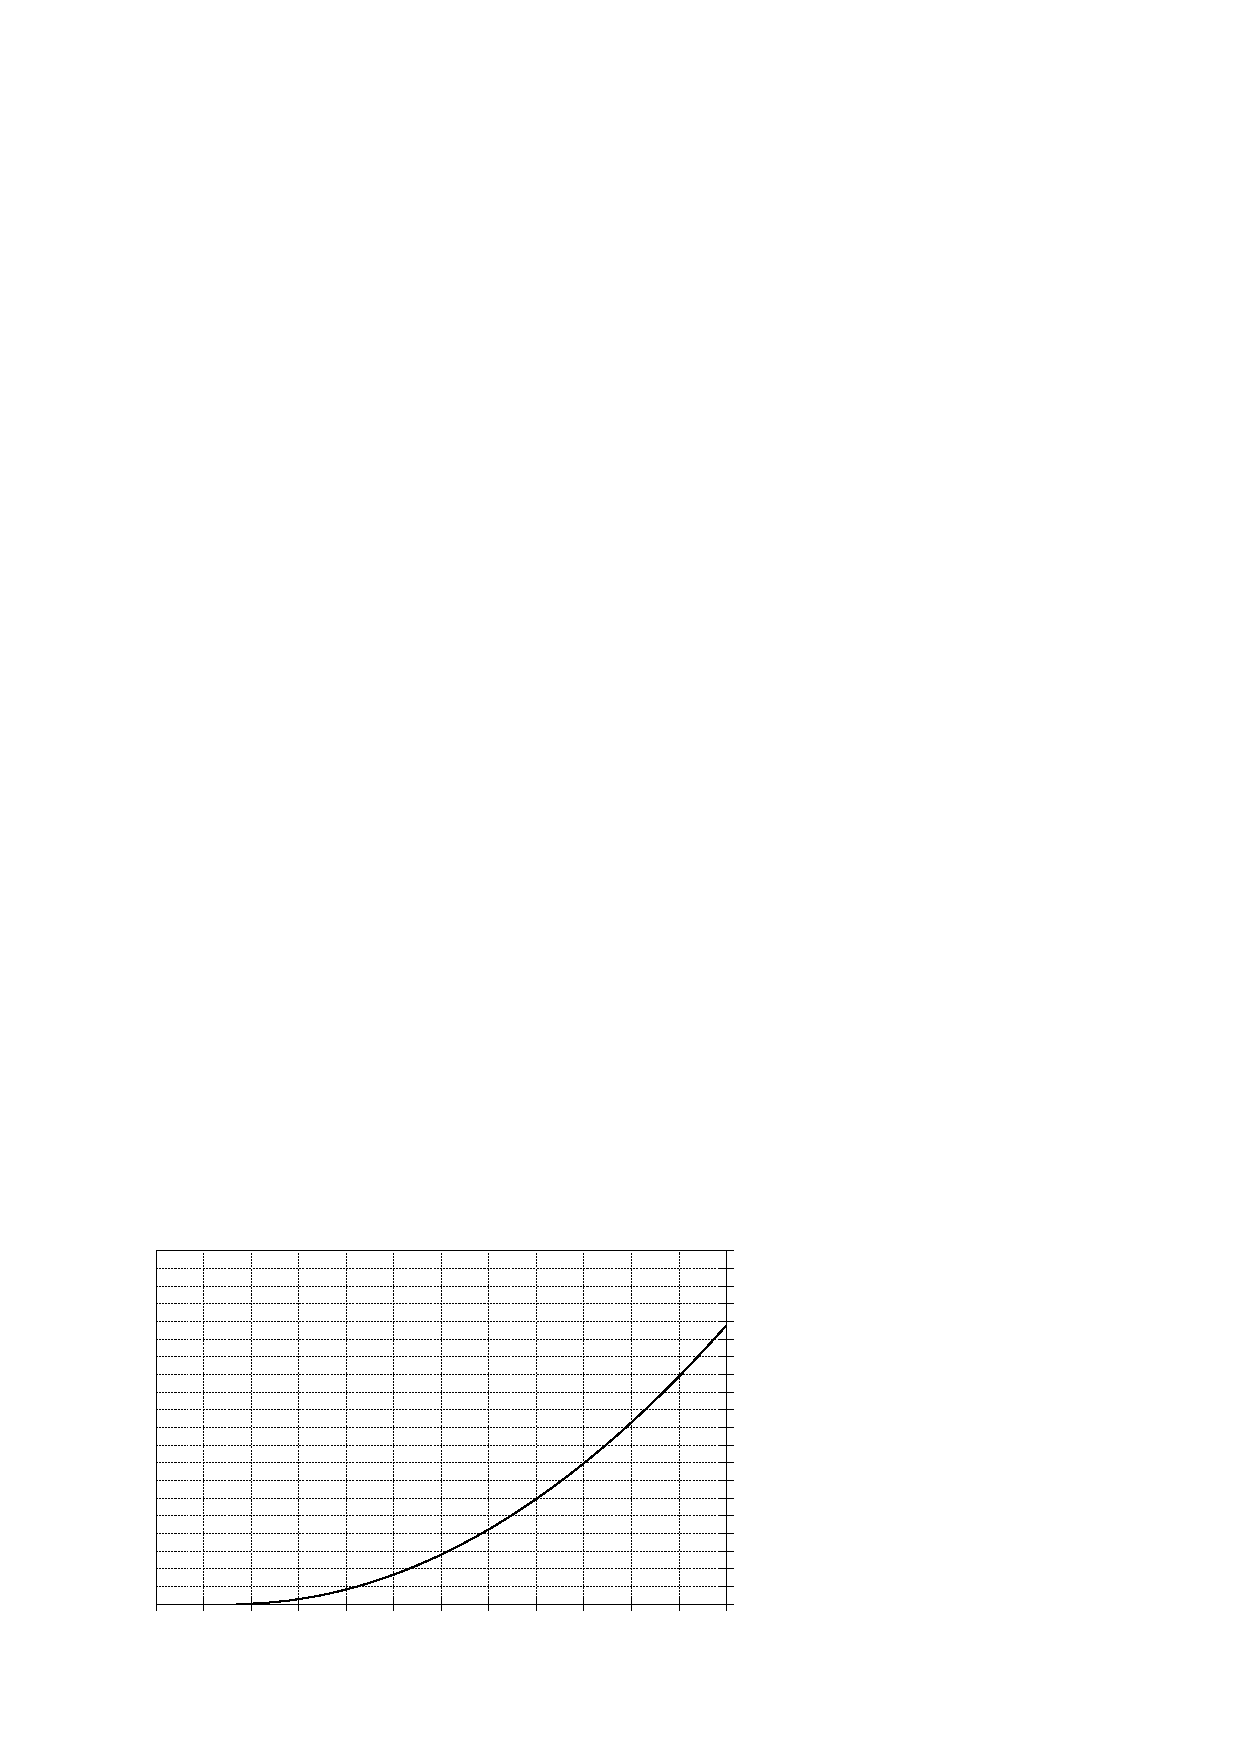
\includegraphics[width={316.80bp},height={201.50bp}]{curva1}}%
    \gplfronttext
  \end{picture}%
\endgroup

    \caption{Curvas características de los transistores JFET.}
    \label{curva01}
\end{figure}

